% Created 2023-11-26 Sun 11:01
% Intended LaTeX compiler: pdflatex
\documentclass[11pt]{article}
\usepackage[utf8]{inputenc}
\usepackage[T1]{fontenc}
\usepackage{graphicx}
\usepackage{longtable}
\usepackage{wrapfig}
\usepackage{rotating}
\usepackage[normalem]{ulem}
\usepackage{amsmath}
\usepackage{amssymb}
\usepackage{capt-of}
\usepackage{hyperref}
\usepackage{minted}
\author{Victoria Ordonez}
\date{\today}
\title{Braids Introduction}
\hypersetup{
 pdfauthor={Victoria Ordonez},
 pdftitle={Braids Introduction},
 pdfkeywords={},
 pdfsubject={},
 pdfcreator={Emacs 27.1 (Org mode 9.6.12)}, 
 pdflang={English}}
\begin{document}

\maketitle
\tableofcontents



\section{Abstract}
\label{sec:org721ba52}

Braids are a great way to study knots, considering they have a better diagram organization and are simpler to understand in certain cases. In this paper, we will discuss what a braid is, some braid properties, and the braid group. Finally, we will explore how knots and links relate to braids with Alexander's Theorem and Markov's Theorem.


\section{Braids}
\label{sec:org6ba68c3}
\subsection{Introduction}
\label{sec:org20fec53}
The  best way to  visualize a braid is to imagine a cube, B, whose coordinates in \(\mathbb{R}^{3}\) can be defined as followed: $$ B = \{(x,y,z)|0 \leq x,y,z \leq 1\}$$ At the top of the cube and at the base of the cube, we will mark \(n\) points, \(A_{1},...,A_{n}\) and \(A^{'}_{1}, ... ,A^{'}_{n}\), respectively. Let , $$A_{1} =\left(\frac{1}{2}, \frac{1}{n+1},1 \right), ... , A_{n} = \left( \frac{1}{2}, \frac{n}{n+1},1 \right)$$
$$A^{'}_{1} =\left(\frac{1}{2}, \frac{1}{n+1},0\right), ... ,A^{'}_{n} = \left(\frac{1}{2},\frac{n}{n+1},0 \right) $$

\begin{center}
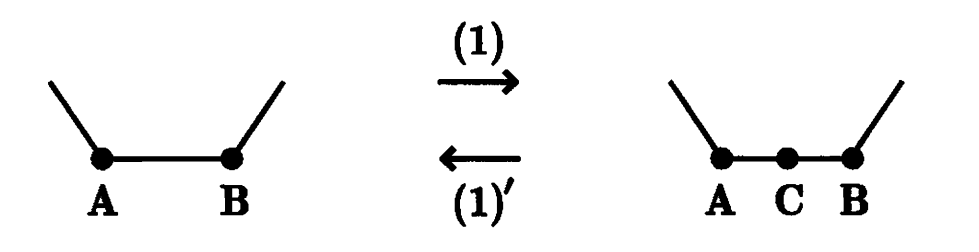
\includegraphics[width=.9\linewidth]{/home/victoria/Pictures/knotpaper/1.png}
\end{center}
$$\caption{Figure \: 2.1.1: \: Cube \: B  \;[3]}$$
 These points will act as fixed endpoints at the top and bottom of the cube, which we will join with \(n\) polygonal arcs. \(A_{1},...,A_{n}\) to \(A^{'}_{1}, ... ,A^{'}_{n}\) are joined with \(n\) polygonal arcs, such that: \(\\  \\\)
 \(\indent \textcircled{1}\) The joined polygonal arcs do not mutually intersect each other \(\\ \\\)
 \(\indent \textcircled{2} A_{i}\) to \(A_{j}\) cannot be joined \(\\ \\\)
 \(\indent \textcircled{3} A_{i}\) to \(A^{'}_{i}\) don't have to be joined, meaning \(A_{i}\) can be joined to \(A^{'}_{j} \\ \\\)
 \(\indent \textcircled{4}\) If we were to take any plane,\(E\), that's parallel to the top and bottom of the cube, \(E\) should intersect each polygonal arc at one and only one point. \(\\ \\\)

    \begin{center}
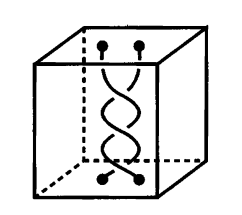
\includegraphics[width=.9\linewidth]{/home/victoria/Pictures/knotpaper/2.png}
\end{center}
    $$\caption{Figure \: \: 2.1.2: \: 2-Braid \; [3]}$$
You can think of \(\textcircled{4}\) as stating that the polygonal arcs cannot go down the cube and then back up, considering that if that were to happen a plane \(E\) would intersect the arc at more than one point. Let's call these polygonal arcs, strings. After dividing \(B\) by \(E\), we can say these \(n\) strings in \(B\) are an \(n-braid\). \(\\\) 

\subsection{Regular Diagram of Braid}
\label{sec:org9ba3f12}
Just like with knots, it is easier to work with projections of n-braids than the actual braid. Therefore, in order to obtain a regular diagram of the braid we can project it onto the \(y-z\) plane. Figure 2.2.1 is the projection of Figure 2.4.2 onto the \(y-z\) plane. 

\begin{center}
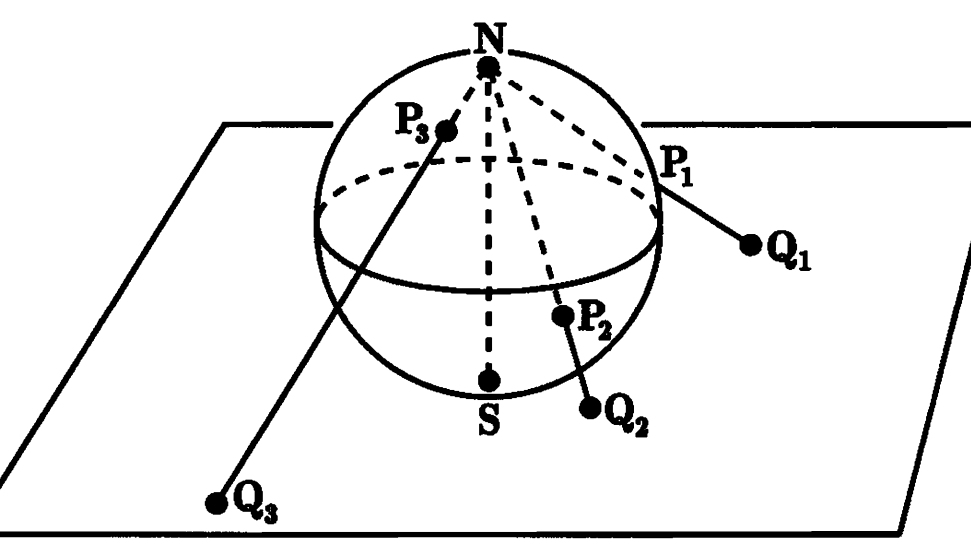
\includegraphics[width=.9\linewidth]{/home/victoria/Pictures/knotpaper/5.png}
\end{center}
$$\caption{ Figure \; 2.2.1: \; Regular \; Diagram \; of \; Figure  \; 2.2.2 \; [3]}$$
\subsection{Trivial n-Braid}
\label{sec:org7e1617a}
We will later see in section 4.2 that we can use the 1-strand trivial braid to create the unknot, so in a way, just like there exists the unknot, there also exists the trivial braid. 
If we were to connect \(A_{1}\) to \(A^{'}_{1}\), \(A_{2}\) to \(A^{'}_{2}\), \ldots{}, \(A_{n}\) to \(A^{'}_{n}\),with straight strings, we would get the trivial n-braid:

\begin{center}
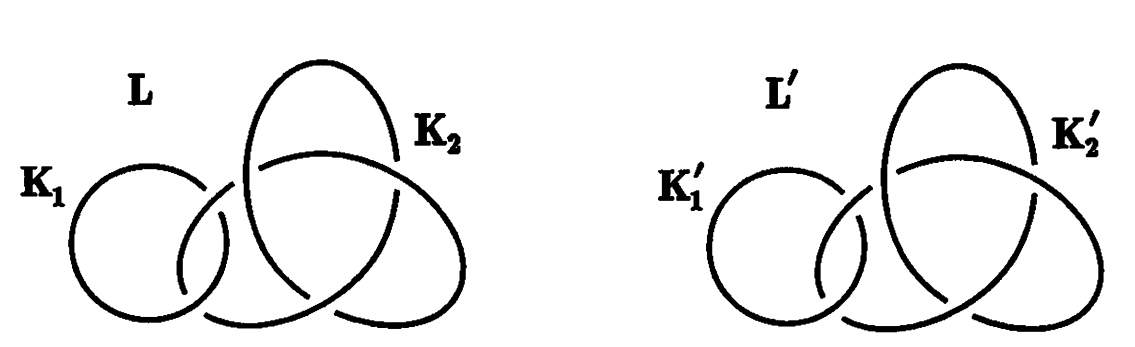
\includegraphics[width=.9\linewidth]{/home/victoria/Pictures/knotpaper/6.png}
\end{center}
$$\caption{Figure \; 2.3.1: \; Trivial \; n-Braid \; [3]}$$
\subsection{Elementary Moves \& Braids}
\label{sec:orgcf7e0eb}
Suppose we are given two n-braids in a cube. If performing elementary knot moves to the strings of each braid, such that the endpoints remain fixed and the strings remain in the cube, transforms one braid into the other, then the two n-braids are equivalent. 
Figure 2.4.1 shows an example of elementary moves being applied to (a) to demonstrate that it is the trivial 2-braid.

\begin{center}
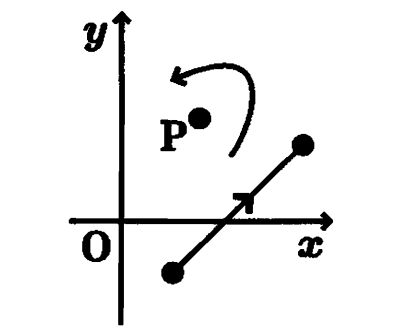
\includegraphics[width=.9\linewidth]{/home/victoria/Pictures/knotpaper/3.png}
\end{center}
$$\caption{Figure \: \: 2.4.1: \: Trivial \: \: 2-Braid \; [3]}$$
Similarly, two braids whose endpoints are fixed can be said to be equivalent if they can continuously be deformed from one to the other without any of the strings intersecting each other as seen in Figure 2.4.2.

\begin{center}
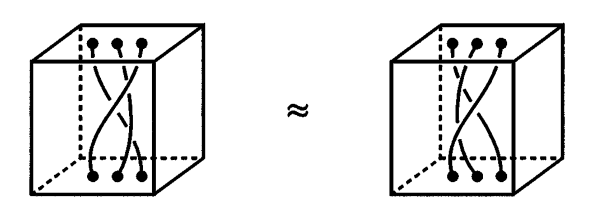
\includegraphics[width=.9\linewidth]{/home/victoria/Pictures/knotpaper/4.png}
\end{center}
$$\caption{Figure \: \: 2.4.2: \: Equivalent \; Braids\; with\; Fixed \; Endpoints \; [3]}$$
\subsection{Braid Permutation}
\label{sec:org046f144}
 Suppose a n-braid, \(\alpha\), has strings connected such that \(A_{1}\) connects to \(A^{'}_{i_{1}}\), \(A_{2}\) connects to \(A^{'}_{i_{2}}\), more generally, \(A_{j}\) connects to \(A^{'}_{i_{j}}\). We can assign \(\alpha\) a permutation: 
 $$\begin{pmatrix}$$
$$1 & 2 & . & . & . & n\\$$
$$i_{1} & i_{2} & . & . & . & i_{n}$$
$$\end{pmatrix}\\$$
$$\caption{Braid \; Permutation \; of \; \alpha}$$
This permutation is called the braid permutation and is a braid invariant. Another way to think about the permutation of a braid is to imagine the first row to be the strings of the braid and the second row to be the endpoints of each of the respective strings. In other words, for \(\alpha\), we know the first string ends up at endpoint \(i_{1}\), the second string ends up at endpoint \(i_{2}\), and so on. Every single braid has a braid permutation. For example: \(\\\)
\(\indent\) The trivial braid (Figure 2.3.1) corresponds to the identity permutation:
   $$\begin{pmatrix}$$
$$1 & 2 & . & . & . & n\\$$
$$1 & 2 & . & . & . & n$$
$$\end{pmatrix}\\$$
$$\caption{Identity \; Permutation}$$
\(\indent\) The braid in Figure 2.1.2 has the braid permutation:
$$ \begin{pmatrix}$$
$$1 & 2\\$$
$$2 & 1 $$
$$\end{pmatrix}$$
$$\caption{Braid \; Permutation \; of \; Figure \; 2.1.2}$$
\section{Braid Group (\(B_{n}\))}
\label{sec:orgc822176}
Let \(B_{n}\) be the set of all n-braids, ie. all the equivalence classes of these braids, where \(n\) is the number of strings in the braids. Just like with every group, the braid group has an operation, an identity element, an inverse, and has associativity under the operation. \(\\ \indent\) The operation of the braid group is the product of two elements in \(B_{n}\), where both elements have the same number of \(n\) strings. In order to define the product of these two elements, let's take two n-braids \(\alpha\) and \(\beta\). Their product, \(\alpha \beta\), will be created by the stacking of  \(\alpha\) vertically on top of \(\beta\), such that the base of \(\alpha\) aligns with the top of \(\beta\). This will create a rectangular solid representing \(\alpha \beta\) that can then be shrunk to keep the original dimensions of \(\alpha\) and \(\beta\), as shown in the figure on the next page.

\begin{center}
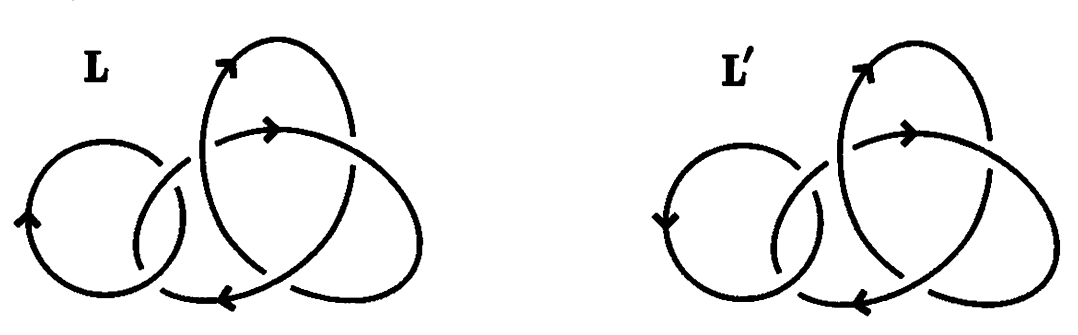
\includegraphics[width=.9\linewidth]{/home/victoria/Pictures/knotpaper/7.png}
\end{center}
$$\caption{Figure \; 3.0.1: \; Product \; of \; two \; 3-Braids \; [3]}$$
 It is important to note that \(\alpha \beta \neq \beta \alpha\), generally. \(\\ \indent\)  We will now show that the action of the product is associative, even though it is not always commutative. Because all we are doing is stacking braids on top of each other and we are not changing the order of the stacking, we are not changing the braid that is being created, meaning \((\alpha \beta) \gamma = \alpha (\beta \gamma)\). This can be seen in Figure 3.0.2 below. However, as mentioned above changing the order in which you stack/multiply your braids does not always create the same braid, so the action of the product is not always commutative.

\begin{center}
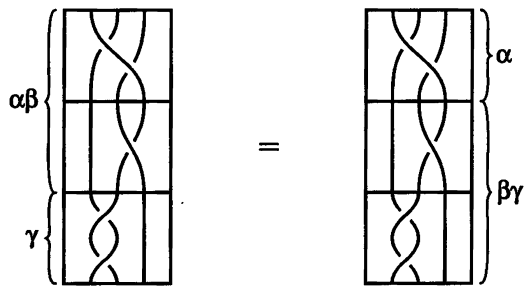
\includegraphics[width=.9\linewidth]{/home/victoria/Pictures/knotpaper/8.png}
\end{center}
$$\caption{Figure \; 3.0.2: \; Associativity \; of \; Braids \; [3]}$$

The identity/unit element of the braid group is simply the trivial braid, considering for any braid \(\alpha\),  \(\alpha e = \alpha = e \alpha\). This is shown in Figure 3.0.3 on the next page. We know this is true, since multiplying \(\alpha\) by \(e\) does not affect \(\alpha\), but rather elongates it, which can be mitigated, considering we can shrink the product of our two braids back to the original size of \(\alpha\). 

\begin{center}
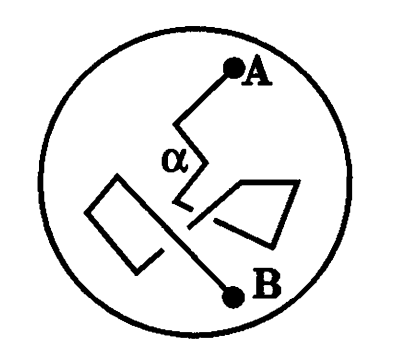
\includegraphics[width=.9\linewidth]{/home/victoria/Pictures/knotpaper/9.png}
\end{center}
$$\caption{Figure \; 3.0.3: \; The \; Trivial \; Braid \; is \; the \; Identity \; [3]}$$
Now to find the inverse element of \(\alpha\), we need to consider the mirror image \(\alpha^{-1}\) of \(\alpha\). Based on this, we know that \(\alpha \alpha^{-1} = e = \alpha^{-1} \alpha\). This is shown in Figure 3.0.4, below.

\begin{center}
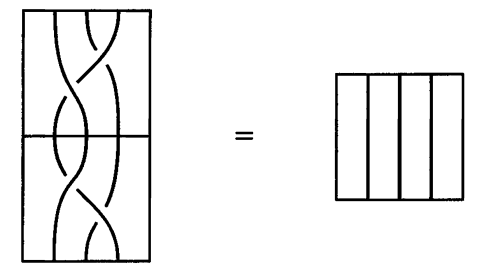
\includegraphics[width=.9\linewidth]{/home/victoria/Pictures/knotpaper/10.png}
\end{center}
$$\caption{Figure \;3.0.4: \; \alpha \alpha^{-1} = e \; [3]}$$
We can tell Figure 3.0.4 is the trivial knot by taking the first string and pulling it to the left, so that the first string ends up being a straight line. The same logic can be applied to the third string and pulling it all the way to the right so that the third string becomes a straight line. Finally, by straightening out the second string we can achieve the trivial knot. We have now discussed all the requirements of the braid group, and I will now introduce the two simplest braid groups: \(\\ \indent\)
   The 1-braid group \(B_{1}\), contains only one element, specifically the trivial braid. Thus, \(B_{1}\) is defined by \(B_{1} = e. \\ \indent\)
   The elements of 2-braid group \(B_{2}\) can be described by the two types of twists, the right twist and the left twist, as shown in Figure 3.0.5 on the next page. 

   \begin{center}
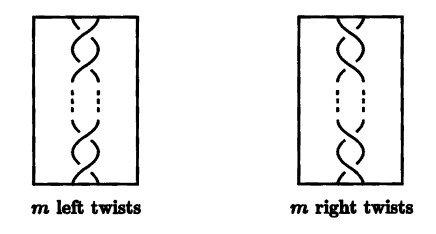
\includegraphics[width=.9\linewidth]{/home/victoria/Pictures/knotpaper/11.png}
\end{center}
$$\caption{Figure \; 3.0.5: \; The \; Two \; Types \;  of \;  Braids \;  in \; B_{2} \; [3] }$$
With any combination of these two types of twists, we will achieve any braid in \(B_{2}\). Therefore, we can also say two 2-braids are equivalent if they have been twisted in the same direction the same number of times. Now that we've started looking at more complex braids, we're going to want a way to describe these braids without drawing the entire diagram. Thus, come in braid generators.
\subsection{Braid Generators}
\label{sec:orgbb42833}
To understand braid generators, let's now divide our braids into rows, such that every row contains only one crossing. We'll start with braids in \(B_{2}\). This can be visualised in our Figure 3.1.1, below

   \begin{center}
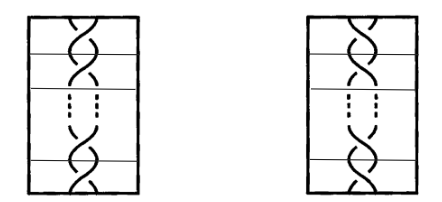
\includegraphics[width=.9\linewidth]{/home/victoria/Pictures/knotpaper/14.png}
\end{center}
   $$\caption{Figure \; 3.1.1: \; Twists \; with \; Rows \; [3] }$$
We will define both of these braids, as having \(m\) twists.  
In our braid on the left, which consists of only left twists, we will see the second strand crossing over the first strand in every row. We will call each of these rows/crossings \(\sigma_{1}\). In our right braid, which consists of only right twists, we will see the first strand crossing over the second strand in every row. We will call each of these rows/crossings \(\sigma_{1} ^{-1}\). Because each of these braids have \(m\) rows/ crossings, we can represent the braid on the left as \(\sigma_{1}^{m}\) and the braid on the right as \(\sigma_{1}^{-m}\). These sigmas are called braid generators, as these two types of crossings are the only ones we need to define any braid. We've now defined the difference between \(\sigma_{1}\) and \(\sigma_{1}^{-1}\), as the difference in the crossings, but what's the difference between \(\sigma_{1}\) and \(\sigma_{2}\). \(\sigma_{1}\) deals with the first two strands of a braid, where as \(\sigma_{2}\) deals with the second strand and the third strand of a braid. Thus, \(\sigma_{1}\) and \(\sigma_{1}^{-1}\) can define \(B_{2}\), but once we reach \(B_{3}\), which has 3 strands, we're going to need \(\sigma_{1},\sigma_{2}\), and their respective inverses. We can generalize \(\sigma_{i}\) by saying that it along with its inverse deal with the \(i^{th}\), and the \(i^{th} +1\) strings, as shown in Figure 3.1.2 below.

  \begin{center}
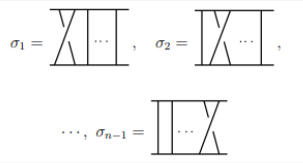
\includegraphics[width=.9\linewidth]{/home/victoria/Pictures/knotpaper/15.png}
\end{center}
  $$\caption{Figure \; 3.1.2: \; Braid \; Generators \; [4]}$$
Let's now look at an example of how braid generators are used to describe braids. Below in Figure 3.1.3, we will see a braid in \(B_{4}\) that can be described by braid generators as \(\sigma_{3}^{-1} \sigma_{1}\sigma_{2}\sigma_{3}\sigma_{2}^{-1}\).

\begin{center}
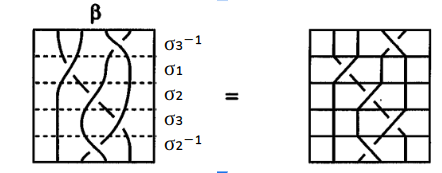
\includegraphics[width=.9\linewidth]{/home/victoria/Pictures/knotpaper/16.png}
\end{center}
$$\caption{Figure \; 3.1.3: \; Using \; Braid \; Generators \; to \; Describe \; a \; Braid \; in \; B_{4} \; [3] }$$
Taking this row by row, we see that the first row deals with third and fourth strand, therefore, we will use either \(\sigma_{3}\) or \(\sigma_{3}^{-1}\) to describe. However, because the third strand is crossing over the fourth strand, it will be \(\sigma_{3}^{-1}\). The second row deals with the first and second strand. Thus, we know we will use either \(\sigma_{1}\) or \(\sigma_{1}^{-1}\). Since the second strand is crossing over the first strand, we know we will use \(\sigma_{1}\). This logic can be applied to the rest of the rows and we can see how \(\sigma_{3}^{-1} \sigma_{1}\sigma_{2}\sigma_{3}\sigma_{2}^{-1}\) describes this braid. 

\subsection{Braid Relations}
\label{sec:orgdd8a7a5}
   \(B_{n}\) is defined by the following presentation:
\[B_n = \left( \sigma_1, \sigma_2, \dots, \sigma_{n-1} \; \biggm| \;  \begin{aligned} \sigma_i\sigma_j &= \sigma_j\sigma_i &&\text{for } |i-j| \geq 2, \\ \sigma_i\sigma_{i+1}\sigma_i &= \sigma_{i+1}\sigma_i\sigma_{i+1} &&\text{for } 1 \le i \le n-2 \end{aligned} \right).\]
As we can see, \(B_{n}\) only needs two types of relations to be defined. The first relation \(\sigma_{i}\sigma_{j} = \sigma_{j}\sigma_{i}\) only applies to \(B_{n \geq 4 }\). This is because the smallest generators that satisfy the condition of this relation are \(\sigma_{1}\) and \(\sigma_{3}\), and \(B_{n}\) only has \(n-1\) generators, so \(\sigma_{3}\) only exists starting from \(B_{4}\). The second relation \(\sigma_{i}\sigma_{i+1}\sigma_{i} = \sigma_{i+1}\sigma_{i}\sigma_{i+1}\) only applies to \(B_{n \geq 3}\). This is again because the smallest generators that satisfy the condition of this relation are \(\sigma_{1}\) and \(\sigma_{2}\), which only exist starting from \(B_{3}\)
\(\\ \indent\) We will now show that the first type of relation is true by looking at Figure 3.2.1. below.

\begin{center}
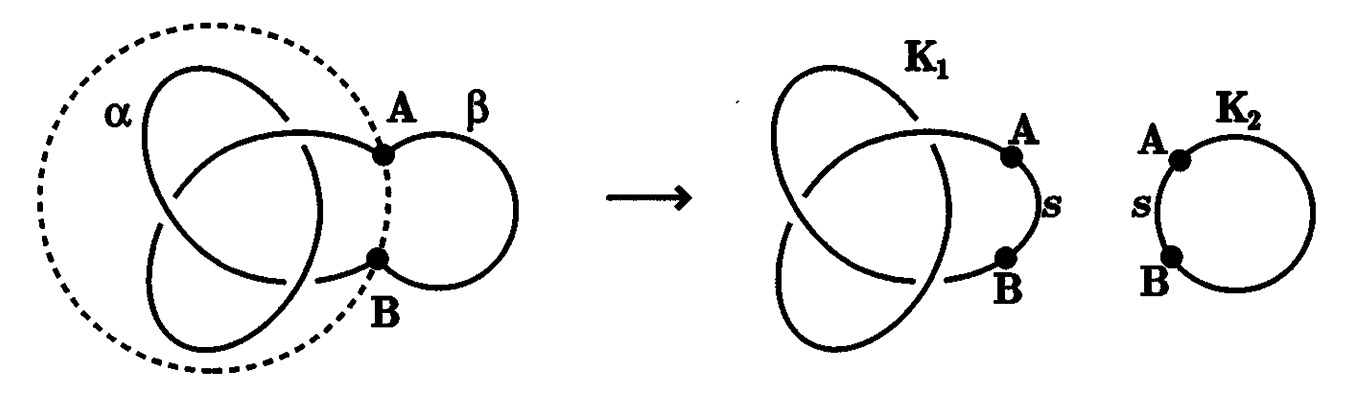
\includegraphics[width=.9\linewidth]{/home/victoria/Pictures/knotpaper/12.png}
\end{center}
$$\caption{Figure \; 3.2.1: \; First \; Braid \; Relation \; [3]}$$
We can see that \(\sigma_{1}\sigma_{3} &= \sigma_{3}\sigma_{1}\) in the figure, since we can squeeze the first twist and second twist in \(\sigma_{1}\sigma_{3}\) down and up, respectively. Likewise, to show \(\sigma_{3}\sigma_{1} &= \sigma_{1}\sigma_{3}\), we can squeeze the first twist and second twist in \(\sigma_{3}\sigma_{1}\) up and down, respectively. Now we will look at the second type of relation on the next page  in Figure 3.2.2.

\begin{center}
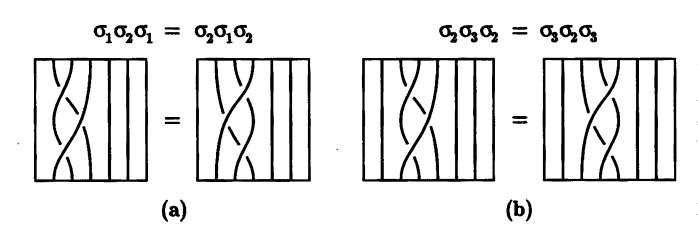
\includegraphics[width=.9\linewidth]{/home/victoria/Pictures/knotpaper/13.png}
\end{center}
   $$\caption{Figure \; 3.2.2: \; Second \; Braid \; Relation \; [3]}$$
   The best way to see that \(\sigma_{1}\sigma_{2}\sigma_{1} &= \sigma_{2}\sigma_{1}\sigma_{2}\)  is to look at \(\sigma_{1}\sigma_{2}\sigma_{1}\). If we take the third strand, and pull it up and to the left, and then take the second strand and pull it down and to the right, we will achieve \(\sigma_{2}\sigma_{1}\sigma_{2}\). Similarly, to show that \(\sigma_{2}\sigma_{1}\sigma_{2} &= \sigma_{1}\sigma_{2}\sigma_{1}\), we will look at \(\sigma_{2}\sigma_{1}\sigma_{2}\) and pull the third strand down and to the right and the second strand up and to the left. These same motions can be applied to show that the second example, \(\sigma_{2}\sigma_{3}\sigma_{2} = \sigma_{3}\sigma_{2}\sigma_{3}\) is true, as well. 


\section{Knots \& Braids}
\label{sec:org677ec37}
\subsection{Braid Closure}
\label{sec:orgd2c27f4}
Let's imagine we have a regular diagram of a braid, by connecting the endpoints of the braid, with parallel arcs, as shown in Figure 4.1.1, we create a closed braid. This closed braid will either be a knot or a link.

\begin{center}
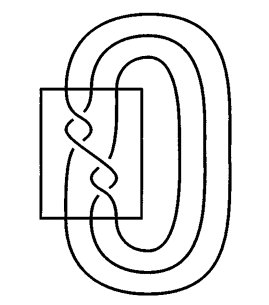
\includegraphics[width=.9\linewidth]{/home/victoria/Pictures/knotpaper/17.png}
\end{center}
$$\caption{Figure \; 4.1.1: \; Closed \; Braid \; [3]}$$
It is important to note that these arcs should connect the endpoints of the braid, such that, an endpoint \(A_{i}\) at the top of the braid has an arc connecting to the endpoint \(A'_{i}\) at the bottom of the braid. Another way to think about this is by looking at Figure 4.1.1. We see that the outermost arc connects endpoint \(A_{1}\) to endpoint \(A'_{1}\), similarly the endpoint \(A_{2}\) is connected to the endpoint \(A'_{2}\), and the endpoint \(A_{3}\) is connected to the endpoint \(A'_{3}\), by the middle and innermost arcs respectively.
\(\\ \indent\) The orientation of the closed braid is usually defined by assigning each string an orientation that starts from \(A_{i}\) and then moving downwards along the corresponding string. Thus, we can create oriented knots or link from braids. 
\subsection{Alexander's Theorem}
\label{sec:orgd1a8459}
Alexander's Theorem states that every knot or link in \(S^{3}\) can be represented as a closed braid.

\begin{center}
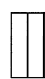
\includegraphics[width=.9\linewidth]{/home/victoria/Pictures/knotpaper/19.png}
\end{center}
$$\caption{Figure \; 4.2.1: \;The \; Trivial \; 1-Braid \; [3]}$$  

One of the simplest examples of showing a knot or link can be represented by a closed braid is by taking the trivial braid and closing it. If the trivial braid has only one string as in Figure 4.2.1, by closing it we create the unknot. If the trivial braid has n-strings as in Figure 2.3.1 , by closing it, we create the n-component unlink.
The proof for Alexander's Theorem is algorithmic and very long and tedious, so I won't explain it here, but I highly suggest reading Birman's proof [5], if that's what you're looking for. 
\subsection{Markov's Theorem}
\label{sec:orgd0c0f70}
   Markov's Theorem states that if B and C are closed braids representing the same isotopy
class of oriented links, then it is possible to transform B into C by a sequence of braid
isotopies and Markov moves (a Markov sequence).

\begin{center}
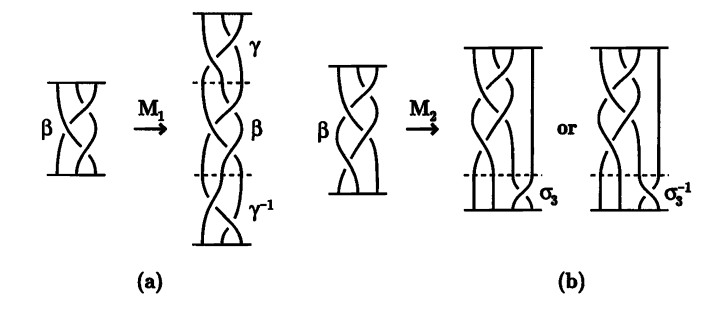
\includegraphics[width=.9\linewidth]{/home/victoria/Pictures/knotpaper/20.png}
\end{center}
$$\caption{Figure \; 4.3.1: \;Markov \; Moves  \; [3]}$$
There are two markov moves, \(M_{1}\) and \(M_{2}\). \(M_{1}\) is the operation that transforms an element, \(\beta\), of the braid group \(B_{n}\) into the n-braid \(\gamma \beta \gamma ^{-1}\), where \(\gamma\) is an element of \(B_{n}\). This can be shown in part a of Figure 4.3.1. As we can see \(\beta = \sigma_{2} \sigma_{1}^{-1} \sigma_{2}\) becomes \(\sigma_{2} \sigma_{1}^{-1} \sigma_{2}\sigma_{1}^{-1}\sigma_{2} \sigma_{2}^{-1}\sigma_{1}\), which is equal to \(\gamma \beta \gamma ^{-1}\), where \(\gamma = \sigma_{2} \sigma_{1}^{-1}\), after \(M_{1}\) is applied.

\(M_{2}\) is the operation that transforms a n-braid, \(\beta\), into either a \(\beta \sigma_{n}\) or a \(\beta \sigma_{n}^{-1}\), (n+1) braid, where \(\sigma_{n}\) is a generator of \(B_{n+1}\). This can be shown in part b of Figure 4.3.2. As we can see \(\beta = \sigma_{2}\sigma_{1}^{-1}\sigma_{2}\sigma_{1}^{-1}\), which is an element of \(B_{3}\) turns into \(\beta\sigma_{n}\) or \(\beta\sigma_{n}^{-1}\), which is an element of \(B_{4}\) after M2. \(\\ \indent\)
Thus, Markov's Theorem allows us to determine when two braids represent the same knot or link. The proof of Markov's Theorem is even longer than the proof for Alexander's Theorem, so again I will not be explaining it here. However, a great proof in terms of seifert circles and reidemeister moves can be found in [6]. 
\section{Conclusion}
\label{sec:orge5898a8}
In this paper, we introduced braids, their properties, and the braid group. We also discuss how closed braids can represent any knot or link, and that there exist moves that allow us to determine when two braids represent the same knot or link. Because the braid group exists, we can study knots algebraically instead of just topologically, which gives us more to work with. There are also other braid invariants that we have not discussed, but that can also be applied to knots, which give us even more resources to study knots, as well. 

\section{References}
\label{sec:org8f755d6}
\begin{enumerate}
\item Jones , V. F. R. (2005). The Jones Polynomial. University of California at Berkely Department of Mathematics.\url{https://math.berkeley.edu/\~vfr/jones.pdf}. \(\\ \\\)
\item Jones , V. F. R. (2014). The Jones Polynomial for Dummies. University of California at Berkely Department of Mathematics.\url{https://math.berkeley.edu/\~vfr/jonesakl.pdf}. \(\\ \\\)
\item Murasugi, K., \&amp; Murasugi, K. (2008). The Jones Revolution. In Knot theory and its applications (pp. 217–247). essay, Birkhäuser. \url{https://www.maths.ed.ac.uk/\~v1ranick/papers/murasug3.pdf}. \(\\ \\\)
\item Glasscock, D. (2012, June). What is a braid group? - Ohio State University. Retrieved April 25, 2023, from \url{https://math.osu.edu/sites/math.osu.edu/files/BraidGroup.pdf}  \(\\ \\\)
\item Birman, J. S., \&amp; Brendle, T. E. (2005, February 26). Braids: A survey. arXiv.org. Retrieved April 28, 2023, from \url{https://arxiv.org/abs/math/0409205} \(\\ \\\)
\item Traczyk, P. (1998). A new proof of Markov's braid theorem. Banach Center Publications, 42(1), 409–419. \url{https://doi.org/http://matwbn.icm.edu.pl/ksiazki/bcp/bcp42/bcp42127.pdf}  \(\\ \\\)
\item Kamada, S. (2002). Braid and knot theory in dimension four. Mathematical Surveys and Monographs, 95. \url{https://doi.org/https://www.ams.org/books/surv/095/surv095-endmatter.pdf} \(\\ \\\)
\item Kim, S., \&amp; Manturov, V. O. (2022, June 2). Lecture 6. Alexander's theorem and Markov's theorem - tsinghua university. Retrieved April 28, 2023, from \url{https://ymsc.tsinghua.edu.cn/\_\_local/B/9E/5A/3D8685AA0880367961727C3556C\_7E5D1E08\_77B71.pdf}
\end{enumerate}
\end{document}
